
\section{Zeigerinstrumente ablesen}
\label{section:zeigerinstrumente_ablesen}
\begin{frame}%STARTCONTENT

\begin{columns}
    \begin{column}{0.48\textwidth}
    \begin{itemize}
  \item Richtige Auswahl der zu messenden Größe mit dem Schalter wählen
  \item Richtige Skala anhand des Messbereichs wählen
  \item Ggf. muss um einen Faktor 10 oder 100 multipliziert oder dividiert werden
  \item Vorteil: Man sieht kontinuierliche Änderungen
  \end{itemize}

    \end{column}
   \begin{column}{0.48\textwidth}
       
\begin{figure}
    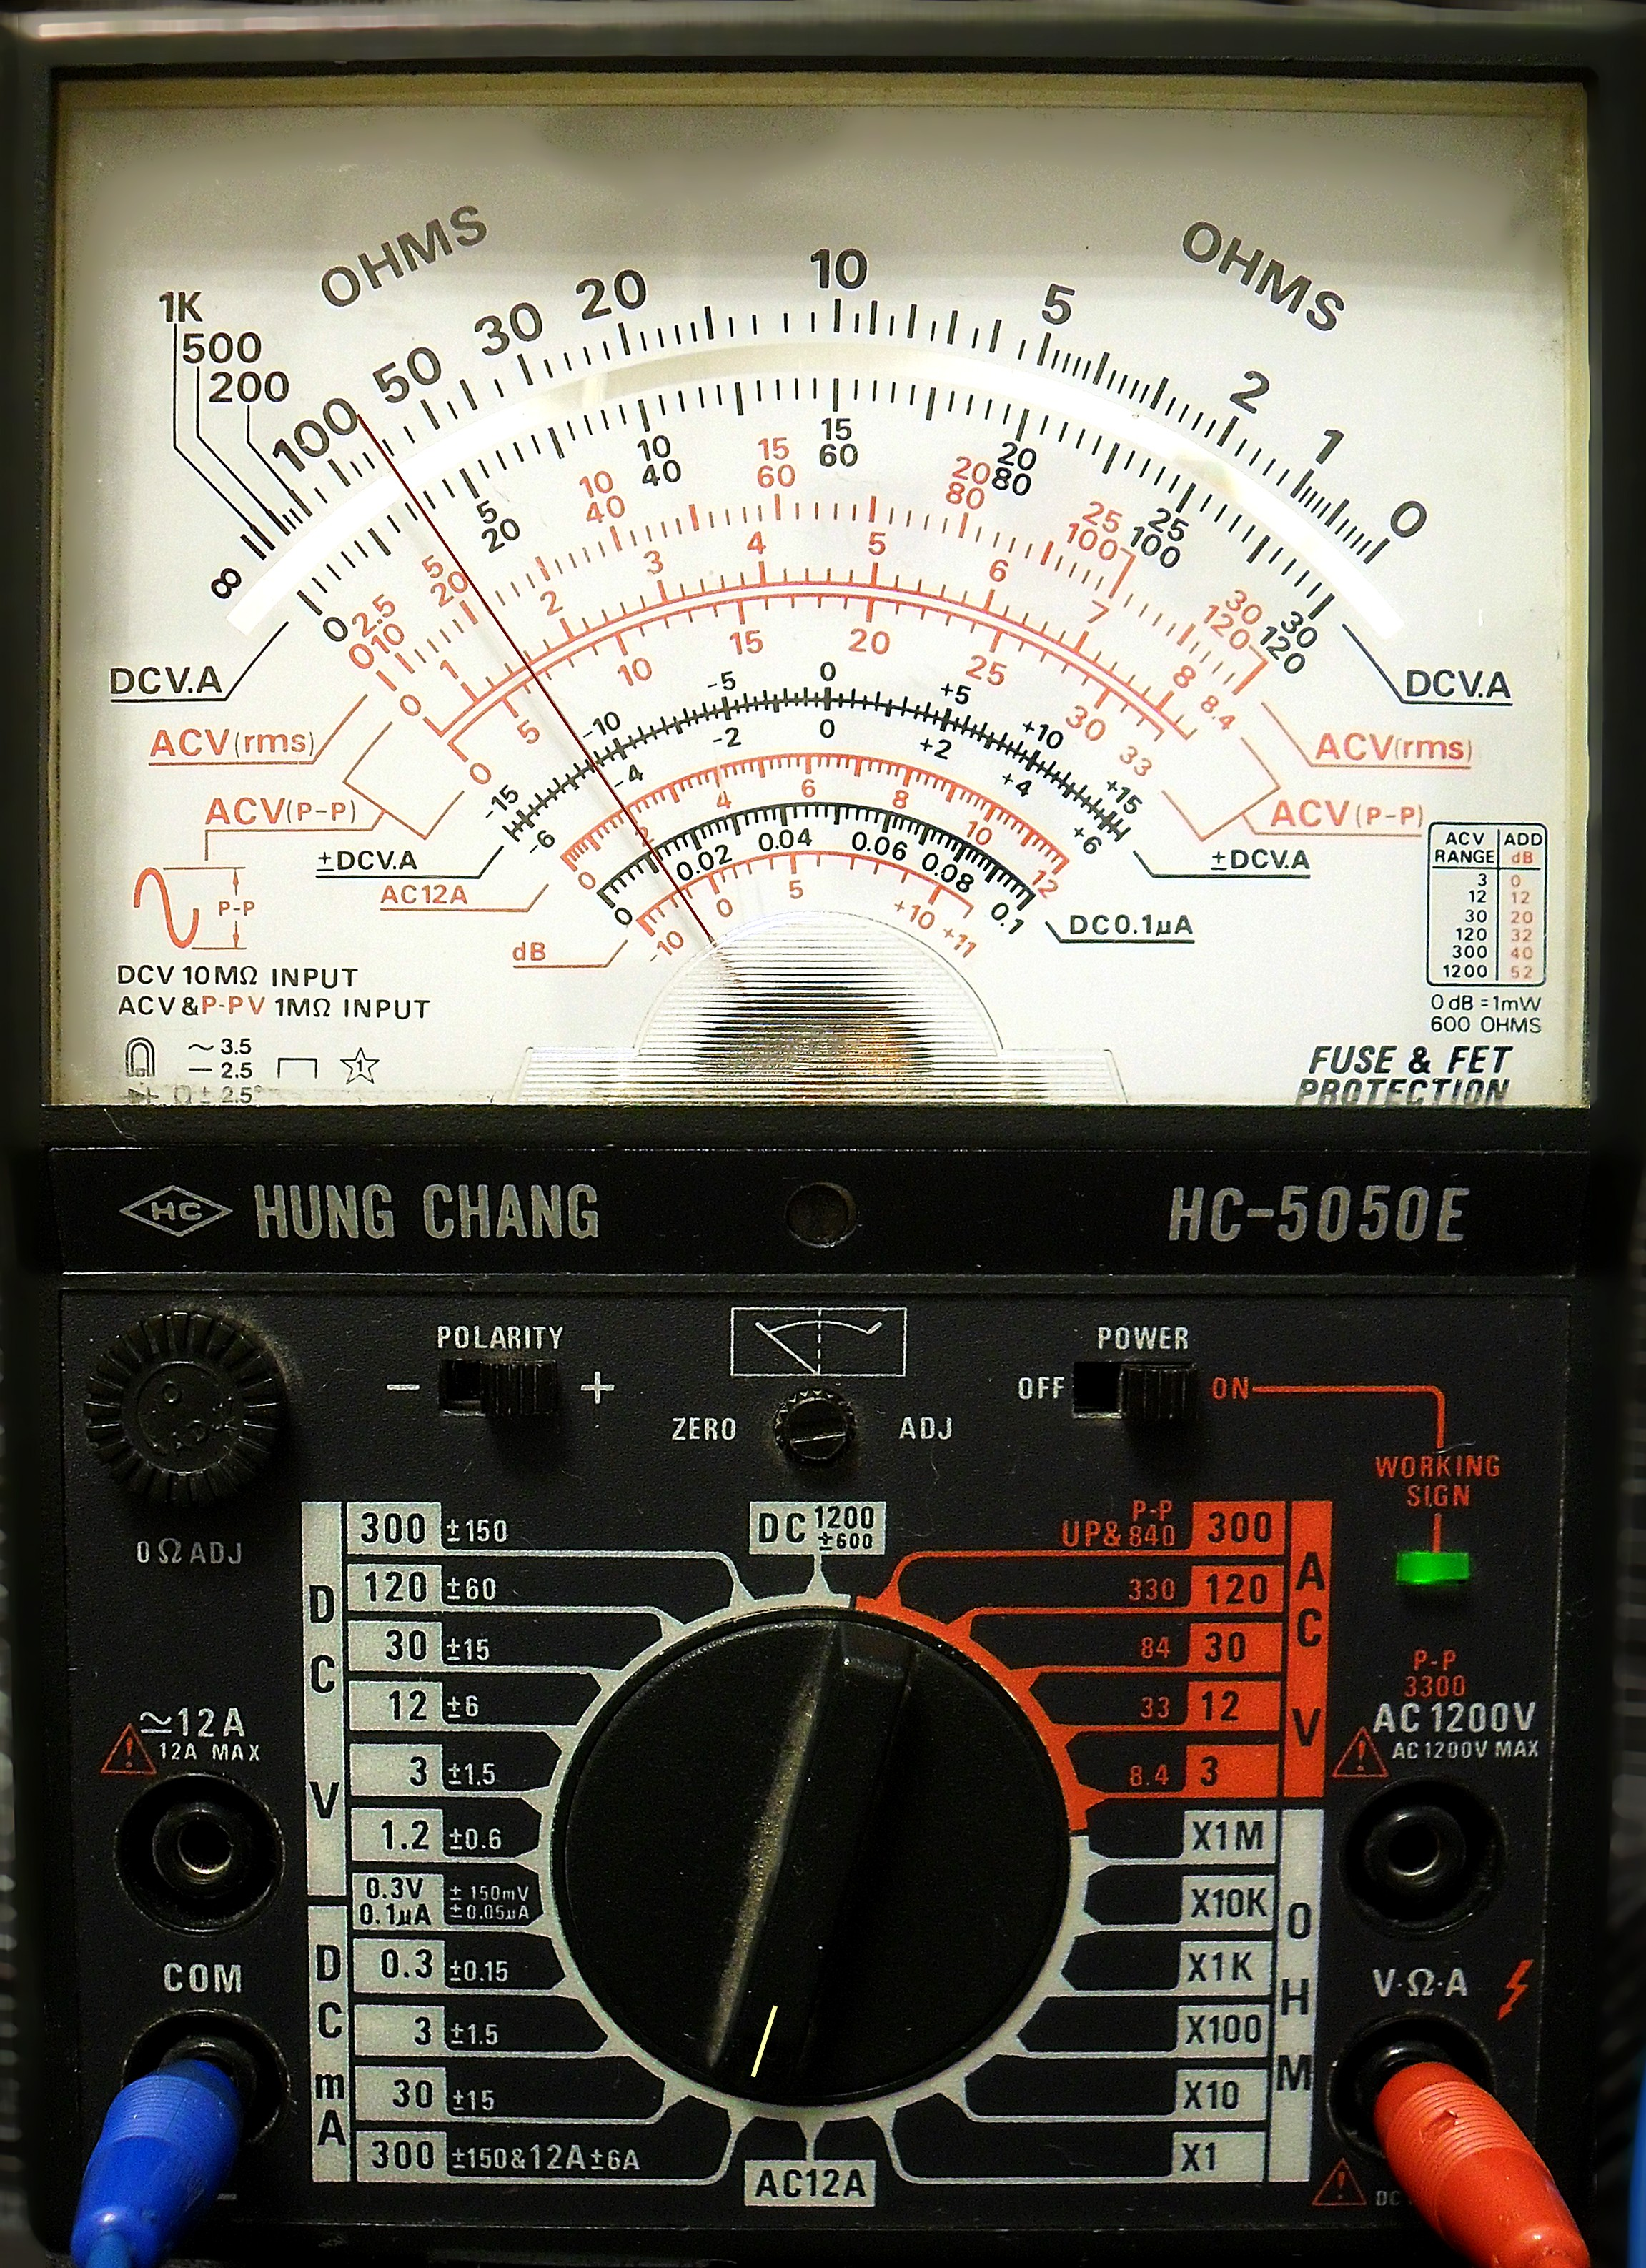
\includegraphics[width=0.85\textwidth]{foto/197}
    \caption{\scriptsize Zeigerinstrument mit mehreren Skalen}
    \label{e_zeigerinstrument}
\end{figure}

   \end{column}
\end{columns}

\end{frame}

\begin{frame}
\frametitle{Parallaxenfehler}
\begin{columns}
    \begin{column}{0.48\textwidth}
    \begin{itemize}
  \item Parallaxenfehler vermeiden, indem gerade drauf geschaut wird
  \item Viele Zeigerinstrumente haben einen Spiegel hinter dem Zeiger
  \item Wenn der Zeiger sich im Spiegelbild überdeckt, wird gerade drauf geschaut
  \end{itemize}

    \end{column}
   \begin{column}{0.48\textwidth}
       
\begin{figure}
    \includegraphics[width=0.85\textwidth]{foto/196}
    \caption{\scriptsize Zeigerinstrument mit Spiegel und Parallaxenfehler beim Ablesen}
    \label{e_parallaxenfehler}
\end{figure}

   \end{column}
\end{columns}

\end{frame}

\begin{frame}
\only<1>{
\begin{PQuestion}{EI103}{Welche Spannung wird bei dem folgenden Messinstrument angezeigt, wenn dessen Messbereich auf \qty{10}{\V} eingestellt ist? }{\qty{8,8}{\V}}
{\qty{29}{\V}}
{\qty{2,9}{\V}}
{\qty{88}{\V}}
{\DARCimage{1.0\linewidth}{41include}}\end{PQuestion}

}
\only<2>{
\begin{PQuestion}{EI103}{Welche Spannung wird bei dem folgenden Messinstrument angezeigt, wenn dessen Messbereich auf \qty{10}{\V} eingestellt ist? }{\qty{8,8}{\V}}
{\qty{29}{\V}}
{\textbf{\textcolor{DARCgreen}{\qty{2,9}{\V}}}}
{\qty{88}{\V}}
{\DARCimage{1.0\linewidth}{41include}}\end{PQuestion}

}
\end{frame}

\begin{frame}
\only<1>{
\begin{PQuestion}{EI104}{Welche Spannung wird bei dem folgenden Messinstrument angezeigt, wenn dessen Messbereich auf \qty{300}{\V} eingestellt ist?}{\qty{290}{\V}}
{\qty{29}{\V}}
{\qty{8,8}{\V}}
{\qty{88}{\V}}
{\DARCimage{1.0\linewidth}{41include}}\end{PQuestion}

}
\only<2>{
\begin{PQuestion}{EI104}{Welche Spannung wird bei dem folgenden Messinstrument angezeigt, wenn dessen Messbereich auf \qty{300}{\V} eingestellt ist?}{\qty{290}{\V}}
{\qty{29}{\V}}
{\qty{8,8}{\V}}
{\textbf{\textcolor{DARCgreen}{\qty{88}{\V}}}}
{\DARCimage{1.0\linewidth}{41include}}\end{PQuestion}

}
\end{frame}%ENDCONTENT
